\documentclass[tiny]{corsage}

\usepackage[T1]{fontenc}
\usepackage[spanish]{babel}
\usepackage{amssymb}
\usepackage{amsmath}
\usepackage{hyperref}
\usepackage{indentfirst}
\usepackage{tcolorbox}
\usepackage{xcolor}

\newcommand{\R}{\mathbb{R}}
\newcommand{\Tri}{\text{Tri}}
\newcommand{\segment}[1]{\overline{#1}}

\definecolor{definition-line}{HTML}{FF4040}
\definecolor{definition-background}{HTML}{FFE0E0}

\hypersetup{
    pdftitle={3ds min 2026},
    pdfauthor={Autodesc}
}

\makeatletter
\newcommand*{\@doendeq}{%
	\everypar{{\setbox\z@\lastbox}\everypar{}}%
}
\makeatother

\newcommand{\rest}{%
	\par
	\vspace{0.5\parskip}%
	\begin{center}%
		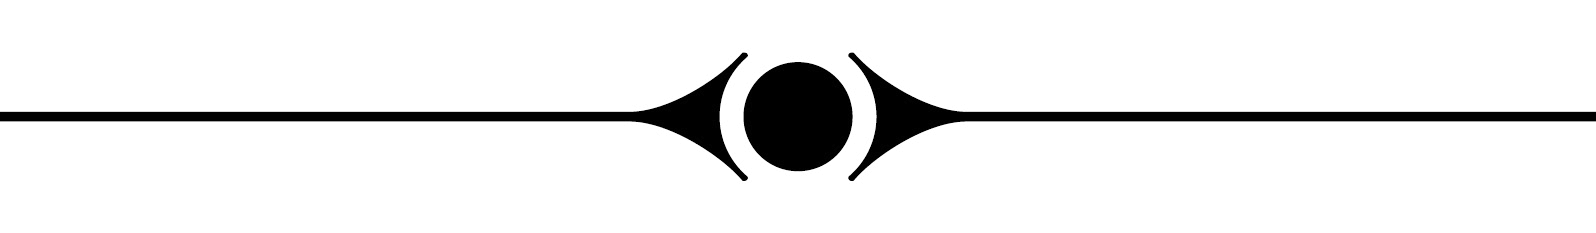
\includegraphics[width=0.2\linewidth]{rest}%
	\end{center}%
	\vspace{-\parskip}%
	\ignorespacesafterend\par\noindent\aftergroup%
}

\newcommand{\pant}{%
	\par
	\vspace{0.5\parskip}%
	\begin{center}%
		\centerline{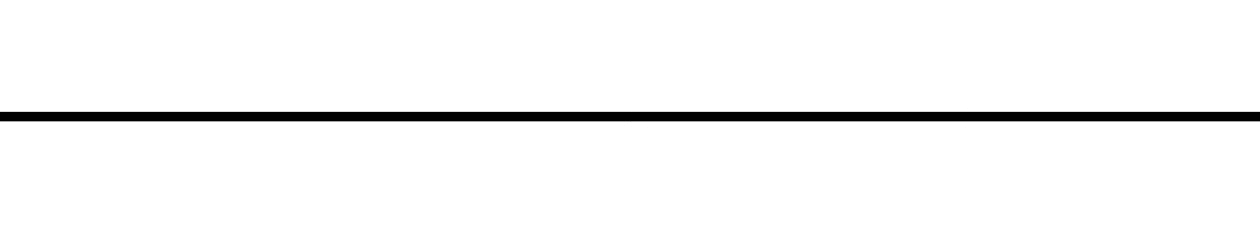
\includegraphics[width=0.15\linewidth]{pant}}
	\end{center}%
	\vspace{-\baselineskip}%
	\par\ignorespacesafterend\noindent\aftergroup%
}

\makeatletter
\newenvironment{definition}{%
	\begin{tcolorbox}[
		left skip=0.5cm,
		right skip=0.5cm,
		left=8pt,
		right=8pt,
		top=3\parskip,
		bottom=2\parskip,
		colback=definition-background,
		colframe=definition-line,
		boxrule=0pt,
		leftrule=4pt,
		sharp corners=all
	]%
}{%
	\end{tcolorbox}%
	\ignorespacesafterend\par\noindent\aftergroup\@doendeq%
}

\makeatother

\begin{document}
\section{Definición del enunciado}
	Considere un polígono convexo $P = \langle v_0, v_1, v_2, \dots, v_{n - 1} \rangle$ con $n$ lados $\segment{v_0v_1}$, $\segment{v_1,v_2}$, $\dots$, $\segment{v_{n - 1}v_n}$,  donde $v_n = v_0$.  Dados dos vértices no adyacentes $v_i$ y $v_j$, llamamos al segmento $\segment{v_iv_j}$ una \emph{cuerda} del polígono.

	Una \emph{triangulación} del polígono $P$ es un conjunto $T$ que lo divide en triángulos disjuntos.  En una triangulación, las cuerdas no se intersecan salvo en los vértices, y el conjunto $T$ es maximal:  Cada cuerda no perteneciente a $T$ interseca alguna cuerda de $T$.  Los lados de los triángulos producidos por la triangulación son o bien cuerdas pertenecientes a $T$ o lados del polígono.  Dado un mismo polígono, existen múltiples formas de triangularlo.

	Dados un polígono $P = \langle v_0, v_1, v_2, \dots, v_{n - 1} \rangle$ y una función peso definida sobre los triángulos formados por una triangulación $w: \Delta(i, j, k) \to \R$, el \emph{problema de la triangulación óptima} consiste en encontrar una triangulación que minimice la suma de los pesos de todos los triángulos pertenecientes a la triangulación.

	Proponemos para este trabajo usar la siguiente función peso, que corresponde a calcular el perímetro del triángulo:
	\begin{equation}
		w(\Delta{v_iv_jv_k}) = \left | \segment{v_iv_j} \middle | + \middle | \segment{v_jv_k} \middle | + \middle | \segment{v_kv_i} \right |
		\label{fn-w}
	\end{equation}

	Dada una cuerda $\segment{v_iv_j}$ sobre el polígono $P$, quedan trazados dos \emph{subpolígonos} $P_{i, j} = \langle v_i, v_{i + 1}, v_{i + 2}, \dots, v_j \rangle$ y $P_{j, i} = \langle v_j, v_{j + 1}, v_{j + 2}, \dots, v_i \rangle$.  Nuestro problema es encontrar, dado un polígono convexo $P$ con $n$ lados y una función peso $w$:
	\begin{equation}
		\mathbb{S} = \min{\left \{ \sum_{i = 0}^{n - 3}{w(T_i)} \ \middle | \  T \in \Tri(P) \right \}}
		\label{def-sol}
	\end{equation}

	De donde $\Tri(P)$ es el conjunto de todas las posibles triangulaciones para el polígono $P$.

\section{Demostración}

\section{Tésis principal}
	puto

	\[ \sigma = \sum_{k = 1}^n{f(h_k) \cdot \Delta x_k} \]

	\[ \mathbb{T}odos\ \mathbb{P}utos \] 
	\[especialmente\ \mathbb{FELIPE\ ISERN} \]


\end{document}
